\chapter{Resultaten en reflectie}
\label{ch:results_reflection}
\section{Behaalde resultaten}
In dit hoofdstuk volgt een objectieve beoordeling op de resultaten van dit onderzoek. \\

Het resultaat van deze bachelorproef zijn een paar zaken:

\begin{enumerate}
	\item Een literatuuronderzoek naar de huidige stand van zaken en een grondige beschrijving van het probleem
	\item Methodologie: Een opsomming van en onderzoek naar technologieën die enerzijds samen passen en anderzijds een positieve invloed hebben op ons probleem
	\item Een proof-of-concept van een digitale assistent
	\item De beoordeling van een advocaat van Deltalex en zodoende feedback over de impact op zijn workflow
\end{enumerate}

\subsection{Literatuurstudie}
De literatuurstudie is goed verlopen en de documenten gevonden zijn relevant en up-to-date.
De onderzoeksvraag is in subvragen verdeeld en individueel onderzocht en er is onderzoek gedaan naar mogelijke oplossingen voor ieder probleem.

\subsection{Methodologie}
De technologieën gevonden zijn open-source, up-to-date en lokaal inzetbaar.
Dit maakt ze ideaal voor de implementatie van een proof-of-concept dat 100\% lokaal kan draaien.
Iedere technologie is besproken maar relatief oppervlakkig onderzocht.
Langdurig gebruik van de applicatie zal hun waarde uitwijzen.

\subsection{Proof-of-concept}
Het geleverde proof of concept is een fork van een veelgebruikt chatplatform, gebouwd m.b.v. het LangChain framework.
Dat maakt het een geteste oplossing die performant is out-of-the box als je in de cloud deployt.
De aanpassing van de app gebeurde met trial and error maar is uiteindelijk in orde gekomen.
Het embedding model heeft krachtig en snel zijn werk gedaan.
Het large-language model heeft soms wat moeite met spelling en kan soms wel eens hallucineren (foute informatie verzinnen),
maar de gegenereerde resultaten dienen louter ter inspiratie voor een advocaat om zijn werk op te baseren.

\section{Beoordeling proof-of-concept}


\subsection{Voorbeeldprompt en persoonlijke beoordeling}
\begin{lstlisting}
PROMPT: schrijf een ingebrekestelling voor 5000 euro aan aqualex
ANSWER:

	Ingebekeringverzoek

	Wij, [Naam en adres van de gemaakte bekering], vroegtelijk aangeduid als De Vermogende Party, op grond van artikel 475 ter, derde lid van het Gerechtelijk Wetboek, 
	hierbij verzoeken aan u, eerder bevoegd gezien bij de familie- rechtbank, een ingebrekestelling te doen van € 5.000,00 aan onze klantenrekening bij uw instelling, 
	onder nummer [Klantnummer], met vermelding dat deze ingebrekestelling gedaan wordt ter behandeling van de nalatenschap van onze overleden klant en volgens ons 
	kennisgevingen bedraagt het netto actief van de nalatenschap niet meer dan € 5.000,00.

	Bij aanvaarding van deze ingebrekestelling, zullen wij onze schulden tegenover uw instelling vervullen en gelijktijdig aan u het geld overmaken dat wordt gevorderd door de ingebrekestelling.

	Als de verwerper of verwerpers van de nalatenschap op eer verklaren dat volgens hun kennis het netto actief van de nalatenschap niet meer 
	bedraagt dan € 5.000,00, wordt deze ingebrekestelling uitgeoefend en vervult onze schulden aan uw instelling. 
	In geval dit geen geval is, zal ons verzoekschrift worden overweegd op de wijze omschreven in artikel 1231-4, tweede lid van het Gerechtelijk Wetboek.

	Wij danken u voor uw ondersteuning en verwachten u binnen een week te horen over de uitvoering van deze verzoekschrift.

	Voorzichtig en met zorg,
	[Naam en adres van de gemaakte bekering]
\end{lstlisting}
\newpage
Minpunten:
\begin {itemize}
\item Veel spelfouten
\item Waarschijnlijk totaal verkeerde verwijzingen naar wetsartikels
\item Relatief kort voor dergelijk document
\end{itemize}

Pluspunten:
\begin{itemize}
	\item Professionele schrijfstijl
	\item Parameters worden schijnbaar niet in de wind geslagen en correct gebruikt
\end{itemize}

\subsection{Beoordeling van een advocaat van Deltalex}
Volgende pagina geeft een screenshot weer van de beoordeling. 
\begin{figure}
	\makebox{
		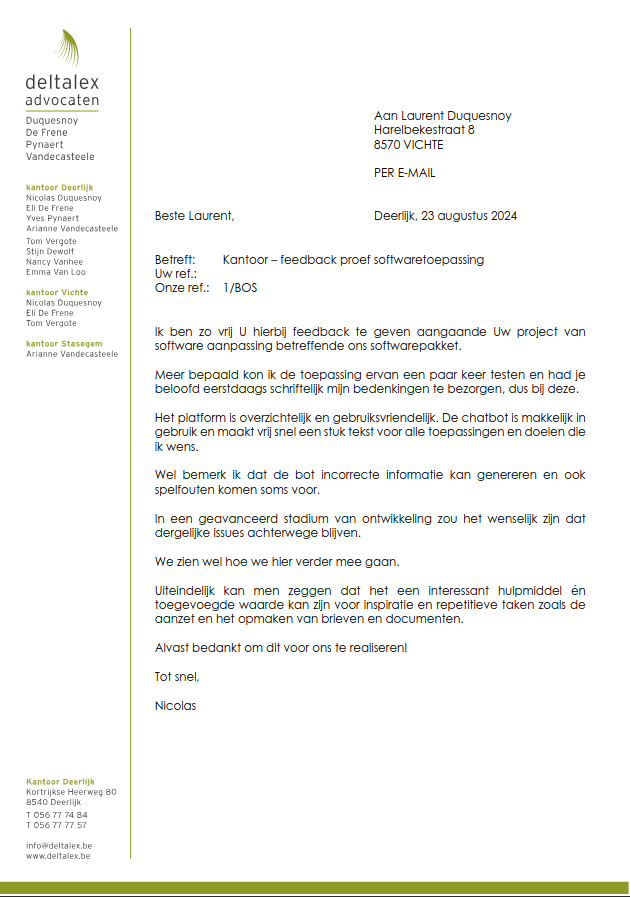
\includegraphics{feedback.png}
	}
	\captionof{figure}{Een screenshot van een brief gestuurd ter evaluatie van Deltalex Chat}
\end{figure}

\newpage
\section{Reflectie}
Een reflectie verloopt heel goed aan de hand van auto-evaluatie d.m.v. vragen die men aan zichzelf stelt.
Hieronder volgen een paar vragen die kunnen ontspringen wanneer men denkt aan automatisatie van workflows en repetitieve taken.\\

\textbf{Welke taken zijn er nu makkelijk te automatiseren?}
De taken die hier in deze bachelorproef beschreven worden gaan over:
\begin{itemize}
	\item \textbf{Opzoekingswerk verrichten in documentendatabases}
	\item \textbf{Opzoekingswerk verrichten in publieke databases}
	\item \textbf{Opstellen van documenten}
\end{itemize}
Een digitale assistent kan een advocaat helpen met deze taken te versnellen door tekst te genereren ter inspiratie en met relevante informatie uit een database.
Het opstellen en gebruiken(versturen, indienen bij de rechtbank, ...) van deze documenten moet nog altijd gebeuren door de advocaat zelf.
Een digitale assistent dient niet ter vervanging van een advocaat, maar wel als een tool die hun workflow kan versnellen. \\

\textbf{Hoeveel productiviteitswinst kan een advocaat realiseren bij deze taken?}
Het gebruik van een digitale assistent zal opzoekingswerk versnellen en dienen ter inspiratie.
Om nog efficiënter te kunnen werken kan een advocaat technieken leren zoals sneltoetsen en tools gebruiken zoals browserextensies om hun workflow exponentieel te optimaliseren.
Hoeveel productiviteitswinst er dan is, hangt af van advocaat tot advocaat.
Sommigen zullen hun workflow bewaren zoals hij is en zijn er tevreden mee.
Anderen zullen altijd op zoek zijn om deze te versnellen en te optimaliseren en kunnen zich hier ook actief mee bezighouden.
Indien men de tijd wil vrijmaken om hier onderzoek naar te verrichten, zal er over de tijd een gestage stijging
zijn in de snelheid van hun workflow door het gebruik van technieken en digitale assistenten. \\

\textbf{Waarmee moet men rekening houden bij de ontwikkeling van een digitale assistent?}
Het belangrijkste aspect bij de ontwikkeling van een digitale assistent bij een advocatenkantoor is waarschijnlijk dataveiligheid.
Er mag absoluut, in geen enkele instantie twijfel ontstaan bij de gebruiker of bij de cliënt dat er vertrouwelijke data op het spel staat.
Een dergelijk voorval zou potentieel destructief zijn voor de klantenrelaties en het imago van het advocatenkantoor.
Andere belangrijke aspecten zijn gebruikersvriendelijkheid, snelheid van tokengeneratie en de kwaliteit van de gegenereerde antwoorden.\\

\textbf{Wat zijn de voor- en nadelen van een automatie via chatbots?}
De voordelen van chatbots zijn de snelheid van antwoorden, de bijna menselijke manier van interactie en de bron van inspiratie voor het opstellen van documenten.
Chatbots zoals ChatGPT zijn de laatste jaren aan een gigantische opmars bezig en hun functionaliteiten worden alleen maar beter dankzij de gigantisch hoge graad van evolutie in de technologische sector.
Nadelen van chatbots kunnen dingen zijn zoals hallucinatie(generatie van incorrecte antwoorden), grammaticale repetitie, ...
Het is altijd aangeraden om hun output te valideren i.p.v. er blind op te vertrouwen.

\section{Verbeteringen en aanpassingen EP3}
\begin{itemize}
	\item Bijna volledige rewrite van corpustekst(buiten literatuurstudie en reflectie)
	\item Proof-of-concept toegevoegd
	\item Dankzij POC feedback van een advocaat ontvangen en toegevoegd
	\item Veel gerichtere technologiekeuze, geavanceerder dan eerste iteratie bachelorproef waar onderzoek puur hypothetisch was
\end{itemize}
